\section{Qualità di processo}
Per garantire la qualità del progetto si utilizza come riferimento lo standard ISO/IEC 12207:1995. Dopo uno studio dettagliato di tale documento sono stati scelti i processi\ap{G}
ed, in alcuni casi, anche le loro rispettive attività trattate anch'esse come dei processi\ap{G} vista la loro importanza. Il tutto è stato semplificato ed adattato in base alle 
esigenze del progetto. Come è previsto nello standard tutti i processi\ap{G} scelti sono ordinati nei macro processi\ap{G}: primari, di supporto ed organizzativi. Ognuno di essi fa parte 
di un processo\ap{G} intermedio e proprio per questo motivo è possibile vedere la sua appartenenza nella sezione: Processo\ap{G} di riferimento.

\subsection{Processi primari}
Sono i processi\ap{G} e le attività che fanno parte dello sviluppo del software e hanno lo scopo di soddisfare tutti i requisiti concordati con il cliente.

\subsubsection{Analisi dei requisiti}
    \paragraph{Metrica - Percentuale requisiti soddisfatti}
    \begin{itemize}
        \item \textbf{Codice:} MPC-01
        \item \textbf{Descrizione:} È la percentuale dei requisiti che devono essere soddisfatti.
        \item \textbf{Processo di riferimento:} Sviluppo
        \item \textbf{Sigla:} PRS
        \item \textbf{Formula:} \begin{math}{PRS = {requisiti \; soddisfatti \over requisiti \; totali}\; \cdot \; 100}\end{math}
        \item \textbf{Range di valori che può assumere:}
        \begin{itemize}
            \item \textbf{Accettabile:} 100\%
            \item \textbf{Ottimale:} 100\%
        \end{itemize}
    \end{itemize}

\subsubsection{Progettazione di dettaglio}
    \paragraph{Metrica - Incapsulamento CBO}
    \begin{itemize}
        \item \textbf{Codice:} MPC-02
        \item \textbf{Descrizione:} Il "Coupling Between Objects" misura il numero delle classi correlate ad una classe al di fuori dalla gerarchia di ereditarietà. Più è alto il grado di coupling e più il sistema è difficile da mantenere.
        \item \textbf{Processo di riferimento:} Sviluppo
        \item \textbf{Sigla:} CBO
        \item \textbf{Formula:} \begin{math}{CBO = {\sum_{i=1}^{N} \cdot \; C_i}}\end{math} \\ N = numero classi non appartenenti alla gerarchia di ereditarietà \\ C_i = classe correlata
        \item \textbf{Range di valori che può assumere:}
        \begin{itemize}
            \item \textbf{Accettabile:} 0$\leq$CBO$\leq$4
            \item \textbf{Ottimale:} 0$\leq$CBO$\leq$2
        \end{itemize}
    \end{itemize}

    \paragraph{Metrica - Livello profondità gerarchia}
    \begin{itemize}
        \item \textbf{Codice:} MPC-03
        \item \textbf{Descrizione:} È il valore intero che indica la profondità della gerarchia formata tra classi. Se una gerarchia è formata da una classe allora il valore è uguale a 1.
        \item \textbf{Processo di riferimento:} Sviluppo
        \item \textbf{Sigla:} LPG
        \item \textbf{Range di valori che può assumere:}
        \begin{itemize}
            \item \textbf{Accettabile:} 1$\leq$LPG$\leq$3
            \item \textbf{Ottimale:} 1$\leq$LPG$\leq$2
        \end{itemize}
    \end{itemize}

\subsubsection{Codifica}  
    \paragraph{Metrica - Numero di parametri per metodo} 
    \begin{itemize}
        \item \textbf{Codice:} MPC-04
        \item \textbf{Descrizione:} Un numero elevato di parametri per metodo può indicare il bisogno di ridurre funzionalità associate a tale metodo. Più è grande questo valore e più la possibilità aumenta nel commettere errori progettuali.
        \item \textbf{Processo di riferimento:} Sviluppo
        \item \textbf{Sigla:} NPM
        \item \textbf{Range di valori che può assumere:}
        \begin{itemize}
            \item \textbf{Accettabile:} 0$<$NPM$<$8
            \item \textbf{Ottimale:} 0$<$NPM$<$4
        \end{itemize}
    \end{itemize}

    \paragraph{Metrica - Linee di commento per linee di codice}
    \begin{itemize}
        \item \textbf{Codice:} MPC-05
        \item \textbf{Descrizione:} È il rapporto tra linee di commento e linee di codice. Per le linee di codice si intende Logical SLOC il numero di linee di codice effettive che corrispondono al numero di statement.
        \item \textbf{Processo di riferimento:} Sviluppo
        \item \textbf{Sigla:} LCLC
        \item \textbf{Formula:} \begin{math}{LCLC = {linee \; di \; commento\over linee \; di \; codice}}\end{math}
        \item \textbf{Range di valori che può assumere:}
        \begin{itemize}
            \item \textbf{Accettabile:} LCLC$\geq$0.25
            \item \textbf{Ottimale:} LCLC$\geq$0.30
        \end{itemize}
    \end{itemize}

\subsection{Processi supporto}
Sono i processi\ap{G} e le attività che aiutano gli altri processi\ap{G} nel raggiungimento del successo e nella qualità del progetto.
  
\subsubsection{Implementazione}
    \paragraph{Metrica - Indice di Gulpease}
    \begin{itemize}
        \item \textbf{Codice:} MPC-06
        \item \textbf{Descrizione:} È l'indice di leggibilità di un determinato testo. Calcola la lunghezza delle parole e delle frasi rispetto al numero totale delle lettere. Il valore è un intero da 0 a 100; se esso è inferiore a 80 sarà difficile da leggere per chi ha la licenza elementare, mentre se è inferiore a 40 sarà difficili da leggere per chi ha un diploma superiore.
        \item \textbf{Processo di riferimento:} Documentazione
        \item \textbf{Sigla:} IG
        \item \textbf{Formula:} \begin{math}{IG = 89 + {{300 \; \cdot \; (numero\; delle \; frasi) \; - \; 10 \; \cdot \; (numero \; delle \; lettere)}\over numero \; delle \; parole}}\end{math}
        \item \textbf{Range di valori che può assumere:} accettabile = 40$<$IG$<$100, ottimale = 80$<$IG$<$100
    \end{itemize}

\subsubsection{Garanzia}
    \paragraph{Metrica - Efficacia del processo}
    \begin{itemize}
        \item \textbf{Codice:} MPC-07
        \item \textbf{Descrizione:} Viene indicato se il processo\ap{G} rispetta gli effetti e i risultati voluti. Un processo\ap{G} deve essere efficace\ap{G} al 100\% per garantire la sua qualità.
        \item \textbf{Processo di riferimento:} Garanzia di qualità
        \item \textbf{Sigla:} EP
        \item \textbf{Range di valori che può assumere:} accettabile = 100\%, ottimale = 100\%
    \end{itemize}

\subsubsection{Verifica}
    \paragraph{Metrica - Code coverage}
    \begin{itemize}
        \item \textbf{Codice:} MPC-08
        \item \textbf{Descrizione:} È la percentuale di copertura del codice attraversato dai test rispetto al totale del codice di base. Per dare una misurazione in termini di grandezza si adoperano le linee di codice come riferimento.
        \item \textbf{Processo di riferimento:} Processi\ap{G} di verifica
        \item \textbf{Sigla:} CC
        \item \textbf{Formula:} \begin{math}{CC = {linee \; di \; codice \; percorse \; dai  \; test \over linee \; di \; codice \; totali} \; \cdot \; 100}\end{math}
        \item \textbf{Range di valori che può assumere:} accettabile = 80\%, ottimale = 100\%
    \end{itemize}

\subsection{Processi organizzativi}
Sono i processi\ap{G} e le attività che coprono gli aspetti organizzativi e di gestione delle risorse.

\subsubsection{Pianificazione}
    \paragraph{Metrica - Schedule variance}
    \begin{itemize}
        \item \textbf{Codice:} MPC-09
        \item \textbf{Descrizione:} È il valore che indica se si è in linea (=0), in anticipo($>$0) oppure in ritardo($<$0) rispetto alla schedulazione delle attività di progetto pianificate nella baseline\ap{G}.
        \item \textbf{Processo di riferimento:} Gestione
        \item \textbf{Sigla:} SV
        \item \textbf{Formula:} \begin{math}{SV = {BCWP \; - \; BCWS}}\end{math} \\BCWP = Budgeted Cost of Work Performed (valore delle attività eseguite nella data corrente) \\BCWS = Budgeted Cost of Work Scheduled (costo pianificato per la realizzazione delle attività di progetto alla data corrente)
        \item \textbf{Range di valori che può assumere:} accettabile = 0, ottimale $>$ 0
    \end{itemize}

    \paragraph{Metrica - Budget variance}
        \begin{itemize}
            \item \textbf{Codice:} MPC-10 
            \item \textbf{Descrizione:} È il valore che indica se la data corrente si è speso di più ($>$0) o di meno($<$0) rispetto a quanto pianificato dal budget totale.
            \item \textbf{Processo di riferimento:} Gestione
            \item \textbf{Sigla:} BV
            \item \textbf{Formula:} \begin{math}{BV = {BCWS \; - \; ACWP}}\end{math} \\BCWS = Budgeted Cost of Work Scheduled (costo pianificato per la realizzazione delle attività di progetto alla data corrente) \\ACWP = Actual Cost of Work Performed (costo effettivamente sostenuto alla data corrente) \\B_tot = Budget totale
            \item \textbf{Range di valori che può assumere:} accettabile = 0$\leq$BV$<$ACWP, ottimale = 0$\leq$BV$\leq$B_tot
        \end{itemize}

\newpage
\subsection{Tabella metriche dei processi}
    \rowcolors{2}{grigetto}{white}
    \renewcommand{\arraystretch}{1.5}
    \begin{longtable}{ c C{4cm} c c c}
    \rowcolor{darkblue}
    \textcolor{white}{\textbf{Metrica}} & \textcolor{white}{\textbf{Nome}} & \textcolor{white}{\textbf{Sigla}} & \textcolor{white}{\textbf{Valore Accettabile}} & \textcolor{white}{\textbf{Valore Ottimale}}\\
    MPC-01 & Percentuale Requisiti Soddisfatti & PRS & PRS=100\% & PRS=100\% \\
    MPC-02 & Coupling Between Objects & CBO & 0$\leq$CBO$\leq$4 & 0$\leq$CBO$\leq$2 \\
    MPC-03 & Livello Profondità Gerarchia & LPG &  1$\leq$ LPG $\leq$ 3 &  1$\leq$ LPG $\leq$ 2\\
    MPC-04 & Numero di Parametri per Metodo & NPM & 0$<$NPM$<$8 & 0$<$NPM$<$4 \\
    MPC-05 & Linee di Codice per Linee di Commento & LCLC & LCLC$\geq$0.25 & LCLC$\geq$0.30 \\
    MPC-06 & Indice di Gulpease & IG & 40$<$IG$<$100 & 80$<$IG$<$100 \\
    MPC-07 & Efficacia del Processo\ap{G} & EP & EP=100\% & EP=100\%  \\
    MPC-08 & Code Coverage & CC & CC=80\% & CC=100\%  \\
    MPC-09 & Schedule Variance & SV & SV=0 & SV$>$0  \\	
    MPC-10 & Budget Variance & BV & 0$\leq$BV$<$ACWP  & 0$\leq$BV$\leq$B_tot  \\	

    \end{longtable}

\subsection{Ciclo di Deming}
    La norma ISO/IEC 12207 utilizza il ciclo di miglioramento continuo dei processi\ap{G} basato sulla sequenza Plan Do Check Act.

    \begin{figure}[h]
        \centering
        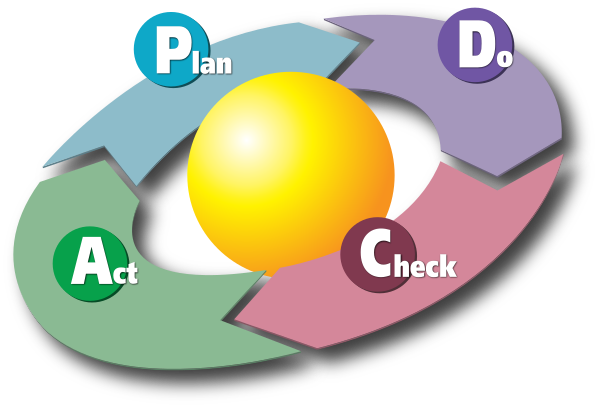
\includegraphics[scale=0.2]{sezioni/Immagini/PDCA.png}
        \caption{PCDA - Plan Do Check Act}
    \end{figure}

    \begin{itemize}
        \item \textbf{Plan}: definisce attività e scadenze necessarie al raggiungimento dei specifici obiettivi di miglioramento;
        \item \textbf{Do}: esegue le attività di "Plan";
        \item \textbf{Check}: verifica l'esito delle azioni di miglioramento rispetto alle attese. Si analizzano i risultati del "Do" e li si confrontano con gli obiettivi individuati nel "Plan";
        \item \textbf{Act}: consolida il tutto e cerca dei metodi per il prossimo miglioramento. Se il "Check" ha dimostrato che il "Plan" implementato dal "Do" è migliore rispetto ai precedenti processi\ap{G} standard, allora questo piano diventa il nuovo processo\ap{G} standard. Altrimenti il vecchio standard in uso rimarrà la baseline\ap{G}.
    \end{itemize}